
\part{Classification Algorithms}
\paragraph{Classification} 
\begin{itemize}
	\item Input: a database $D = {x_1, x_2, \dots, x_n}$ of tuples, a set of classes $C = {C_1, C_2, \dots, C_m}$
	\item Output: a \textbf{mapping} $f: D\rightarrow C$, where each $x_i$ is assigned to a class. 
\end{itemize}
\section{Generalized Linear Models}
\subsection{Component of GLM}
\begin{itemize}
	\item Random component: identifies \textbf{dependent variable $\mu$} and \textbf{its probability function}
	\item Systematc component: identifies the set of \textbf{explanatory variables -- predictors} ($X_1, \dots, X_k$)
	\item Link function: a \textbf{linear} function that links the dependent variable and all explanatory variables.
	$$g(\mu) = \beta_0 + \beta_1 X_1 + \beta_2 X_2 + \dots + \beta_k X_k$$
\end{itemize}
\subsection{Common Link Functions}
\begin{itemize}
	\item \textbf{Identity Link: linear regression}
	$$g(\mu) = \mu = X\beta$$
	\item \textbf{Logit Link: logistic regression}
	$$g(\mu) = \ln(\frac{\mu}{1 - \mu}) = X\beta $$
	\item \textbf{Log Link: Poisson regression}
	$$g(\mu) = \log(\mu) =  X\beta$$
\end{itemize}
\section{Logistic Regression: Binary Classification}
\begin{itemize}
	\item Idea:	
	\begin{itemize}
		\item Gauss-Markov assumptions need to be fulfilled to implement an OLS-Estimator
		
		$\rightarrow$ more \textbf{generalized models} needed to relax the assumptions for OLS
		
		\item Predicting \textbf{categorical dependent variables}: a \textbf{classification} problem.
		\item Limitation from linear regression in classification:
		\begin{itemize}
			\item prediction values $\hat{y}$ should range within [0, 1], linear regression model prediction \textbf{exceeds this range}.
			\item \textbf{violation of Homoscedasticity}: residuals $e_i$ doesn't have constant variance since the true Y only takes two values(0/1). The distribution of the residuals is no longer a normal distribution.
			\item \textbf{violation of No Autocorrelation}: overall residuals of the model follows a systematic pattern, it's positive on one side and negative on the other side $\rightarrow$ Autocorrelation
		\end{itemize}
	\end{itemize}
\end{itemize}

\subsection{The Logistic Regression Model}
The \textbf{binary} logistic regression model described in \textbf{log odds/logit}:
$$\text{log odds} = \ln(\frac{p(X)}{1 - p(X)}) $$
$$\ln(\frac{p(X)}{1 - p(X)}) = \beta_0 + \beta_1 X + \varepsilon$$
\begin{itemize}
	\item Modeling Input: $X_i$, 0/1
	
		  Output: a Logit-model	  
	\item p(X): probability that Y = 1 given X.
	\item \textbf{log odds / logit}: range ($-\infty, +\infty$), the log-ratio of Y = 1 to Y = 0 given X
\end{itemize}

The logistic regression model described in \textbf{odds}: 
$$odds = \frac{p(X)}{1 - p(X)}$$
$$\frac{p(X)}{1 - p(X)} = e^{\beta_0 + \beta_1 X}$$
\begin{itemize}
	\item \textbf{odds}: range [$0, +\infty$), the ratio of Y = 1 to Y = 0 given X
	\begin{itemize}
		\item p(X) = 0.5, odds = 1
		\item p(X) $< 0.5, \rightarrow 0$, odds $\rightarrow 0$
		\item p(X) $> 0.5, \rightarrow 1$, odds $\rightarrow +\infty$
	\end{itemize}
\end{itemize}

\subsection{The Logistic Function}
$$Pr[Y|X] = p(X) = \dfrac{e^{\beta_0 + \beta_1 X}}{1 + e^{\beta_0 + \beta_1 X}}$$
\begin{itemize}
	\item Prediction Input: $X_i$, $\beta_i$
	
	\textbf{Output: $p(X)$}		 
	
	\item Range p(X): [0,1]
	\begin{itemize}
		\item $\beta_0 + \beta_1 X = 0$:  p(X) = 0.5 
		\item $\beta_0 + \beta_1 X  \uparrow$:  p(X) $\rightarrow 1$
		\item $\beta_0 + \beta_1 X  \downarrow$:  p(X) $\rightarrow 0$
	\end{itemize}
	\item $\beta_0$: regression constant, moves the curve \textbf{left/right}
	\item $\beta_1$: regression slope, defines \textbf{steepness} of the curve. $\beta_1 \uparrow$, steepness $\uparrow$
	\item This can be reformed into the logistic regression model. 
	\item Comparison Linear Model \& Logistic Model(the logistic function):
	\begin{figure}[H]
		\centering
		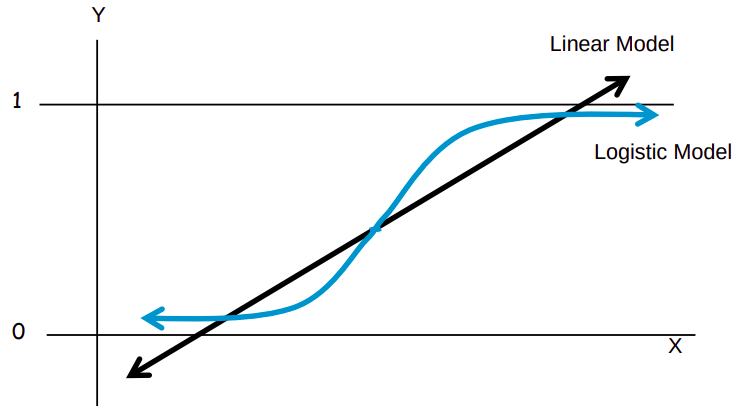
\includegraphics[width=0.6\textwidth]{logit.png}
	\end{figure}
\end{itemize}
Comparison p(X) \& odds \& log-odds:
\begin{figure}[H]
	\centering
	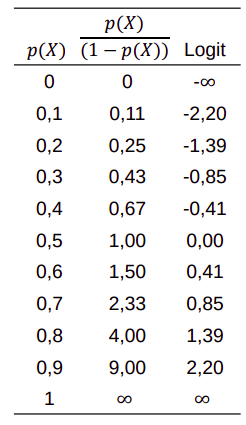
\includegraphics[width=0.25\textwidth]{logodds_odds.png}
\end{figure}

\subsection{Multiple Logistic Regression Model}
$$\ln(\frac{p(X)}{1 - p(X)}) = \beta_0 + \beta_1 X_1 + \beta_2 X_2 + \dots + \beta_k X_k$$
\begin{itemize}
	\item Interpretation of Coefficients $\beta_j$: 
	\begin{itemize}
		\item \textbf{while keeping all other $x_j$ constant}, if $x_{ij}$ increase by 1, the \textbf{log-odds} will increase/decrease by $\beta_j$, or the \textbf{odds} will increase/decrease by $\mathbf{e^{\beta_j}}$.
	\end{itemize}
	\item Test of Multicollinearity: VIF / correlation coefficient
	\item Test of irrelevant variables: Wald-Test (significance of coefficients) 
\end{itemize}

\subsection{Estimation of Coefficients: Maximum Likelihood Estimator}
\subsubsection{Intro}
The probability of one data point $x_i$ can be modeled as \textbf{Bernoulli trial}: 
$$p^{y_i}(1-p)^{1-y_i}$$
The \textbf{likelihood function}:  the \textbf{joint probability} of observing the dependent variable values of random samples. $\rightarrow$ the product of all Bernoulli trials
$$L = \Pi_{i=1} p^{y_i}(1-p)^{1-y_i}$$
The logistic function can also be described as a \textbf{sigmoid function} in form $S(x) = \frac{e^x}{1 + e^x} = \sigma(x)$
$$P(X) = \sigma(\beta_0 + \beta_1 X)$$
\subsubsection{The Likelihood Function and Maximum Likelihood Estimator}
The \textbf{likelihood function for Logistic Regression Model}:
\begin{align*}
	L &= \Pi_{i=1} p^{y_i}(1-p)^{1-y_i} \\
	  &= \Pi_{i=1} \sigma(\beta_0 + \beta_1 X)^{y_i} \cdot (1 - \sigma(\beta_0 + \beta_1 X))^{1-y_i}
\end{align*}

The \textbf{Maximum Likelihood Estimator}: \textbf{maximizes the joint probability} of observing the set of dependent variables of the random samples.
\\ \ \\
Process:
\begin{itemize}
	\item take the log: $$LL = \ln(L) = \Sigma_{i=1} ( y_{i} \ln(p) + (1 - y_i)\ln(1-p))$$
	\item \textbf{maximize} LL: 
	\begin{align*}
		\beta = \arg\max_{\beta}(LL) &= \arg\max_{\beta} [\Sigma_{i=1} ( y_{i} \ln(p) + (1 - y_i)\ln(1-p))] \\
									 &= \arg\max_{\beta} [\Sigma_{i=1} ( y_{i} \ln(\sigma(\beta_0+\beta_1X)) + (1 - y_i)\ln(1-\sigma(\beta_0 + \beta_1X)))]
	\end{align*}
	\item Method: \textbf{Gradient Ascent}
	\begin{figure}[H]
		\centering
		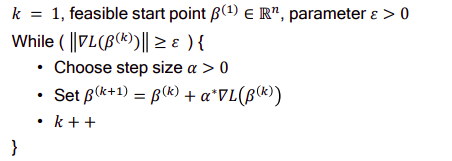
\includegraphics[width=0.65\textwidth]{gradientascent.png}
	\end{figure}
	\begin{itemize}
		\item initial start point
		\item select a step size $\alpha$
		\item compute \textbf{partial derivatives} and \textbf{maximizes the function} $f(x^{(k)} + \alpha \bigtriangledown f(x^{(k)}))$
	\end{itemize}
	\item \textbf{Gradient}(partial derivatives) of the LL-Function: \textbf{chain rule}
	
	 with $z = \beta_0+\beta_1X$
	
	$$\frac{\partial LL}{\beta_j} = \Sigma_{i=1} \frac{\partial LL}{\partial p} \cdot \frac{\partial p}{\partial z} \cdot \frac{\partial z}{\partial \beta_j}$$
	\begin{align*}
		\frac{\partial LL}{\partial p} &= \frac{y_i}{p} - \frac{1 - y_i}{1 - p} \\
		 \frac{\partial p}{\partial z} &= \sigma(z) \cdot(1 - \sigma(z)) \\
		 \frac{\partial z}{\partial \beta_0} &= 1 \text{, } \frac{\partial z}{\partial \beta_j} = x_j\\		 
	\end{align*}
	\begin{align*}
		\frac{\partial LL}{\beta_0} &= \left[ \frac{y_i}{p} - \frac{1 - y_i}{1 - p}\right]  \sigma(z) \cdot(1 - \sigma(z)) = \left[ y_i - \sigma(X\beta) \right] \\
		\frac{\partial LL}{\beta_j} &= \left[ \frac{y_i}{p} - \frac{1 - y_i}{1 - p}\right]  \sigma(z) \cdot(1 - \sigma(z))\cdot x_j = \left[ y_i - \sigma(X\beta) \right] x_j
	\end{align*}
\end{itemize}
\subsection{Quality Metrics of the Model}
\begin{itemize}
	\item \textbf{Null Model}: all predictors $x_i$ has no impact. The model is explained only by the intercept.
	\item \textbf{Fitted Model}: the model is explained by p predictors and 1 intercept.
\end{itemize}

\subsubsection{Null Deviance}
It measures how well the response is explained by \textbf{only the intercept (no predictors)}.
$$\text{null deviance} = -2 \ln(L(null))$$

\subsubsection{Residual Deviance}
$$\text{residual deviance} = -2 \ln(L(fitted))$$
\begin{itemize}
	\item residual deviance $\downarrow$, model quality $\uparrow$
	\item difference between null and residual deviance $\uparrow$, model quality $\uparrow$
\end{itemize}

\subsubsection{AIC}
Additional penalizing term to get a balance between the \textbf{goodness of fit} and \textbf{simplicity of model}.

$$AIC = \text{residual deviance} + 2 \cdot \#\text{parameters in model}$$

\begin{itemize}
	\item AIC $\downarrow$, model quality $\uparrow$
\end{itemize}

\subsubsection{McFadden $\mathbf{R^2}$} the ratio of improvement from null model to fitted model.
$$R_{McFadden}^2 = 1 - \frac{LL(fitted)}{LL(null)} = 1 - \frac{\text{residual deviance}}{\text{null deviance}}$$
\begin{itemize}
	\item model quality $\uparrow$ , LL(fitted) $\ll$ LL(null), $R^2 \rightarrow 1$
	\item model quality $\downarrow$ , LL(fitted) $\approx$ LL(null), $R^2 \rightarrow 0$
	\item rule of thumb: > 0.2 acceptable, > 0.4 ok.
\end{itemize}

\subsubsection{Likelihood Ratio Test}
Does the fitted model explain significantly more variance than null model?
\begin{itemize}
	\item $H_0$: The fitted model explains \textbf{no more variance} than null model
	
	$H_1$: The fitted model explains \textbf{significantly more variance}.
	\item test statistic:
	$$D = -2 \ln (\frac{L(null)}{L(fitted)})$$
	\item Distribution: $\chi^2$-Distribution
\end{itemize}

\subsubsection{Significance Test of Coefficients: Wald Test}
\begin{itemize}
	\item $H_0$: $\beta_i = 0$
	
	$H_1$: $\beta_i \neq 0$
\end{itemize}

\subsubsection{Error Rates}
comparing the predicted classification and the actual classification:
\begin{itemize}
	\item percentage of correct Yes
	\item percentage of correct No
	\item overall percentage of correct predictions
\end{itemize}

\subsection{Model Interpretation}
\subsubsection{R-Result Interpretation}
\begin{figure}[H]
	\centering
	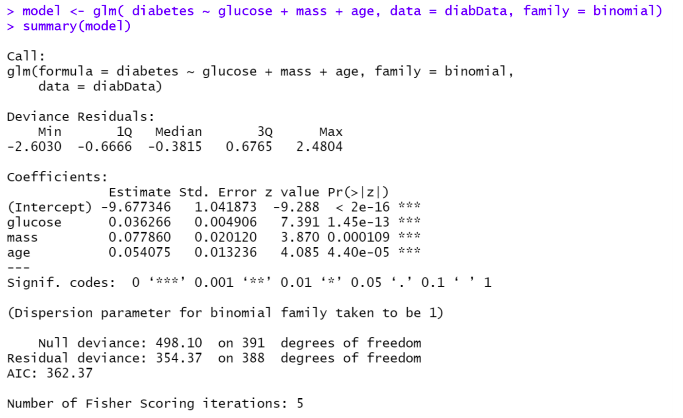
\includegraphics[width=0.75\textwidth]{logit_r.png}
\end{figure}
\begin{itemize}
	\item significance of coefficients: significant if $p < \alpha$ in $\alpha$-level
	\item model: difference between null and residual deviance, AIC
\end{itemize}

\subsubsection{Interpretation of Coefficients}
Effect of change in $x_{ij}$ in \textbf{one unit}:
\begin{figure}[H]
	\centering
	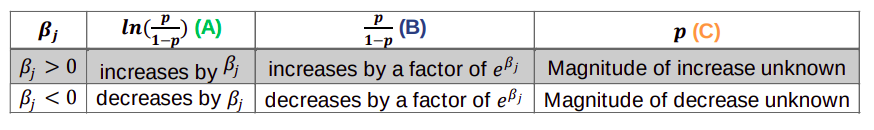
\includegraphics[width=0.9\textwidth]{logit_interpretation.png}
\end{figure}
\begin{itemize}
	\item $\beta_j >0$: 
	\begin{itemize}
		\item If $x_{ij}$ increase by 1, then the \textbf{log odds} will \textbf{increase} by $\beta_j$, or the \textbf{odds} will \textbf{increase} by $\mathbf{e^{\beta_j}}$.
		\item If $x_{ij}$ increase by 1, then the \textbf{log odd ratio} is $\beta_j$, or the \textbf{odd ratio} is $e^{\beta_j}$.
	\end{itemize}
	\item $\beta_j < 0$:
	 \begin{itemize}
	 	\item If $x_{ij}$ increase by 1, then the \textbf{change of log odds} will \textbf{decrease} by $\beta_j$, or the \textbf{change of odds} will \textbf{decrease by a factor} of $\mathbf{e^{\beta_j}}$.
	 	\item If $x_{ij}$ increase by 1, then the \textbf{log odd ratio} is $\beta_j$, or the \textbf{odd ratio} is $e^{\beta_j}$.
	 \end{itemize}
\end{itemize}




\section{Poisson Regression: Binary Classification for Count Data}
\begin{itemize}
	\item Idea: 
	\begin{itemize}
		\item \textbf{count variables (non-negative integers)} as dependent variables
		\item limitation of linear regression / OLS-Estimator
		\begin{itemize}
			\item linear model \textbf{predicts negative values}
			\item count data is often \textbf{highly skewed}: \#crimes committed -- most are 0.
			
			$\rightarrow$ violates normality assumption (residuals follows normal distribution) of OLS-Estimator
		\end{itemize}
	\end{itemize}
	\item Assumption: observed count follows a \textbf{Poisson distribution}.
	$$Pr(y|\mu) = \dfrac{e^{-\mu} \mu^y}{y!}$$
	\begin{itemize}
		\item $\mu$: expected count and expected variance $E(Y) = Var(Y) = \mu$
		\item y: observed count
	\end{itemize} 

	\item Limitation:
	\begin{itemize}
		\item \textbf{Overdispersion}: $E(Y) = Var(Y) = \mu$ not met in real data. 
		
		$\rightarrow$ underestimation of standard errors, potential overconfidence in result. 
		
		$\rightarrow$ Alternative: negative binomial regression
		
		\item \textbf{Zero-inflation}: highly skewed observed data/predictions in 0.
		
		this can't be changed even with negative binomial regression.
	\end{itemize}
	
\end{itemize}
\subsection{Poisson Regression Model}
$$ln(\mu(x)) = \beta_0 + \beta_1 X_1 + \dots \beta_j X_i$$
\subsection{Estimation of Coefficients: Maximum Likelihood Estimator}
The random component(dependent variable) is:
$$Pr(Y|X) = p(X) = \dfrac{e^{-\mu} \mu^y}{y!} = \dfrac{e^{\beta xy} e^{-e^{\beta x}}}{y!}$$

The \textbf{likelihood function}:
$$L(\beta|X,Y) = \Pi_{i=1} p = \Pi_{i=1} \dfrac{e^{\beta x_iy_i} e^{-e^{\beta x}}}{y_i!}$$

The Maximum Likelihood Estimator: 
$$\log L(\beta | X,Y) = \Sigma_{i=1} (\beta x_iy_i - e^{\beta x_i} - \log(y_i!))$$
\begin{itemize}
	\item Method: \textbf{Gradient Ascent}
\end{itemize}
\subsection{Model Interpretation}
R-Result interpretation is same as logistic regression.
\subsubsection{Interpretation of Coefficients}
Effect of change in $X_{ij}$ in \textbf{one unit}:
\begin{figure}[H]
	\centering
	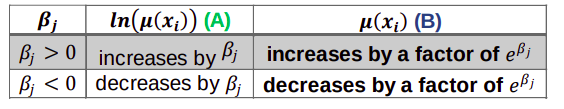
\includegraphics[width=0.65\textwidth]{poisson_coeff.png}
\end{figure}
\begin{itemize}
	\item $\beta_j > 0$: If $x_{ij}$ increases by 1, then the \textbf{log-incidence rate} will \textbf{increase} by $\beta_j$, or the \textbf{incidence rate} will \textbf{increase by a factor} of $e^{\beta_j}$.
	\item $\beta_j < 0$: If $x_{ij}$ increases by 1, then the \textbf{log-incidence rate} will \textbf{decrease} by $\beta_j$, or the \textbf{incidence rate} will \textbf{decrease by a factor} of $e^{\beta_j}$.
\end{itemize}

